\documentclass{article}
\usepackage[utf8]{inputenc}
\usepackage[margin=1in]{geometry}
\usepackage{amsmath}
\usepackage{amsthm}
% Package for making turing machine diagrams %
\usepackage{tikz}
\usetikzlibrary{chains,fit,shapes}
% Packages for algorithms %
\usepackage{algorithm}
\usepackage{algorithmic}
% Package which has the nice looking empty set symbol (\varnothing)
\usepackage{amssymb}
% Package with the ceiling function
%\usepackage{mathtools}
%\DeclarePairedDelimiter{\ceil}{\lceil}{\rceil}
\usepackage{braket}
\usepackage{amsmath} 
\usepackage{amsfonts}
\usepackage{graphicx}
\graphicspath{{/Users/sebastian/Documents/csci3384_conway/figures/}}

\usepackage{amssymb}
\usepackage{comment}
\usepackage{mathtools}
\DeclarePairedDelimiter{\ceil}{\lceil}{\rceil}
\usepackage{bm}

\usepackage{biblatex}
\addbibresource{bibliography.bib}

% Makes table of contents links clickable in pdf readers
\usepackage[colorlinks=true, linkcolor=blue, urlcolor=blue, citecolor=blue, breaklinks=true]{hyperref}

\theoremstyle{definition}
\newtheorem{definition}{Definition}[section]
\newtheorem{problem}{Problem}

\theoremstyle{plain}
\newtheorem{example}{Example}[section]
\newtheorem{exercise}{Exercise}[section]

\theoremstyle{plain}
\newtheorem{fact}{Fact}[section]
\newtheorem{lemma}{Lemma}[section]
\newtheorem{theorem}{Theorem}[section]
\newtheorem{corollary}{Corollary}[section]
\newtheorem{claim}{Claim}[section]

\title{Reachability, Complexity, and the Limits of Conway's Game of Life}
\author{Sebastian Pucher \& Adam Gohain}

\begin{document}

\maketitle

\tableofcontents

\newpage

\section{Introduction: Can Life be Simulated?}
  \textit{    That is the question, isn't it.} For centuries, mathematicians, philosophers, and computer scientists, have spent their lives trying to uncover what it means to truly be alive. Many come together, often crossing their respective disciplines, to construct answers to these larger, often existential questions. Even today, humanity has continued to develop complicated technology in hopes of understanding more about life, how it can be studied, or even how it could possibly be synthesized.

\

\textit{What is life?} Back in 1940, John Von Neumann and Stanislaw Ulam set out to prove an answer to this very question. Von Neumann was an American Mathematician whose research focused on self-replicating systems and cellular automata. Alongside his colleague Ulam, who worked together with Von Neumann on the Manhattan Project, they proposed a simple discrete game that replicated life. Their mathematical model consisted of a two-dimensional grid of square cells, where the state of the next generation of cells would depend on the interaction between living cells and their neighbors \cite{Beginning_Life_2006}. They called it \textit{The Universal Constructor} which produced fascinating properties of time and space usage \cite{Freitas_2004}.

\

Not long after their proposal, a British Mathematician known as John Conway extended upon Ulam and Von Neumann’s research to fabricate an instance of their \textit{Universal Constructor} that better replicated Alan Turing’s model of a “universal computer”. By experimenting with different rules and states between neighboring automata, Conway was able to simplify the model into a game that was only composed of only a few basic rules \cite{Beginning_Life_2006} [see \ref{rules}]. 

\

Shortly after, in 1970, the \textit{Scientific American} published an article articulating how to play the game which resulted in the greatest number of letters reactions from readers at that time \cite{Izhikevich_Conway_Seth}. In the paper, Conway proposed that no initial pattern could grow without limit, and offered fifty dollars to the first person who could disprove him by the end of the year \cite{math-games}. This catalyzed immense popularity in the game, and set forth the many mathematical discoveries that have now been proven about the game, such as its undecidable nature (see section (CITE SECTION)), and recurring patterns [see \ref{patterns}].


\textbf{Going to add a nice image here}

\subsection{The Game}
Similar to how Alan Turing proposed models of computational thinking prior to modern day computers, Conway's Game of Life started as a simple mathematical idea that was “played” on chalkboards and Go boards \cite{Izhikevich_Conway_Seth}. Here are the rules, and how to play: 

\

\textbf{Rules \& Properties: }
\begin{enumerate}
  \label{rules}
  \item \textbf{Domain: }\\ The automata in the game interact within an \textit{infinite} two-dimensional grid of cells. Every cell has eight neighbors \cite{Izhikevich_Conway_Seth}[see \ref{figure_one}]. \label{rule_one}

  \item \textbf{States: }\\ Each automata is represented independently by a single cell which can be either \textit{alive} or \textit{dead}.

  \item \textbf{Initial Configuration: } \\ The beginning set of live or dead cells is determined or ``seeded" by the player prior to any evolution.

  \item \textbf{Evolution: } \\ The following rules are applied to all cells simultaneously in fixed time intervals called \textit{generations} \cite{Bontes2019}.

  \item \textbf{Birth: } \\ A new cell is born at generation $t + 1$ when its state is currently \textit{dead} and has exactly 3 lives neighbors (reproduction) \cite{Bontes2019}.

  \item \textbf{Death: } \\ Any currently living cell will die at generation $t + 1$ if it has less than 2 live neighbors (underpopulation) or more than 3 live neighbors (overpopulation) \cite{Bontes2019}.

  \item \textbf{Persistence: } \\ Any live cell will persist at $t + 1$ if it has 2 or 3 live neighbors at generation $t$ \cite{Izhikevich_Conway_Seth}.
\end{enumerate}

 \begin{figure}[ht]
          \centering
    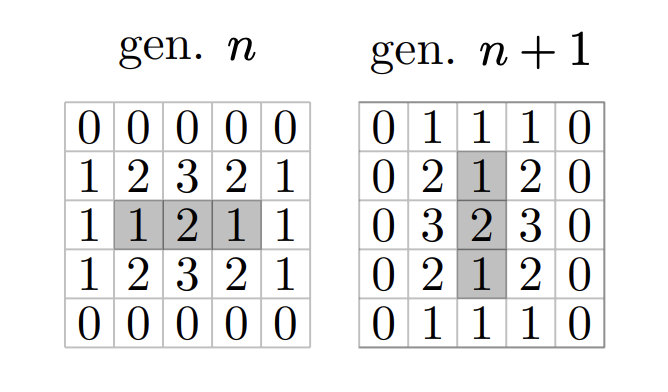
\includegraphics[width=8cm]{figure_one.png}
    \caption{The evolution of a blinker from for 2 generations}
    \label{figure_one}
    \text{J. Bontes. “Searching for patterns in Conway’s Game of Life”}
    \cite{Bontes2019}
\end{figure}

It’s important to note that Conway’s Game of Life is not a game of how we traditionally think of games. There’s no objective, or winning or losing. They’re aren’t even any players – it is known to be a zero player game \cite{Beginning_Life_2006}. As technology advanced, Conway’s Game of Life proved to be well-suited for implementation on computers. Today, the game has been optimized to explore the many unresolved problems the game poses. 

\subsection{So... What's the Big Deal?}

At first glance, Conway’s Game of Life appears to be a simple simulation of cellular life based on just a few rules. However, beneath the surface, the Game hides complexity that has roused intense study since its public release way back in 1970. Decades have been spent examining the self-replicating machines, digital circuits, and unique patterns the Game presents. Another leading interest, of course, is the Game's overall mathematical complexity, which is the main inspiration of this paper. Additionally, many of GoL's difficulties also stem from the Game's Turing Completeness which we also will cover[see section]. 

\ 

\textbf{Proposal}: The purpose of this paper is to both synthesize concrete theoretical mathematics from Complexity Theory into a specific instance of Conway's game of life. More specifically, the paper will be divided into two parts. The first pertaining to the Pattern Reachability Question (PERN), and the second pertaining to Undecidability and Turing Completeness in the game.

\section {Pattern Reachability}
\label{patterns}
One particular challenge within The Game is the difficulty of predicting and discovering the many different patterns (or ``life-forms") that may evolve from one generation to the next. A\textit{ pattern} is defined as a constellation of both live and dead cells that evolve over time \cite{Bontes2019}.

\

Conway's Game of Life is capable of producing patterns that move back and forth, shifting between a finite set of states, patterns that traverse through the grid indefinitely, patterns that trail and leave behind other evolving patterns, and patterns that collide with each other to create other complicated patterns \cite{JG2022conway}.

\

Because of this, there are over a thousand different patterns and life-forms that have been proposed and studied within the Game (many of which are still be discovered today) \cite{Life_Wiki}. Of these many patterns, there are three underlying features that are used to categorize and study them. There are as follows: 

\begin{enumerate}
  \item \textbf{Still Life: } \\ A pattern that remains unchanged from one generation to the next \cite{JG2022conway}.

 \begin{figure}[ht]
          \centering
    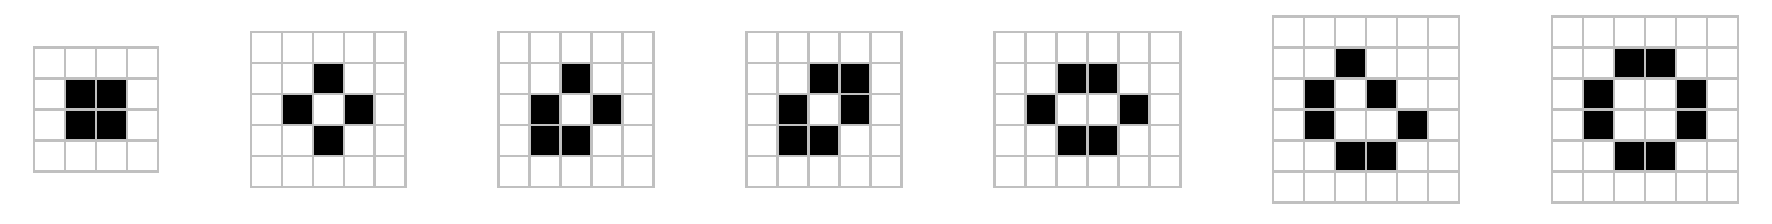
\includegraphics[width=10cm]{figure_two.png}
    \label{stil_lifes}
    \caption{Examples of Still Lifes: From left to right: block, tub, boat, ship, beehive, loaf and pond}
    \text{Nathaniel Johnston and Dave Greene. Conway’s Game of Life: Mathematics and Construction.}
    \cite{JG2022conway}
\end{figure}


  \item \textbf{Oscillator: } \\ A pattern that cycles between finitely many different configurations. The configuration of the pattern within an individual generations is called a \textbf{phases}. The smallest number of generations needed to repeat the cycle is called the \textbf{period} \cite{JG2022conway}.



 \begin{figure}[ht]
          \centering
    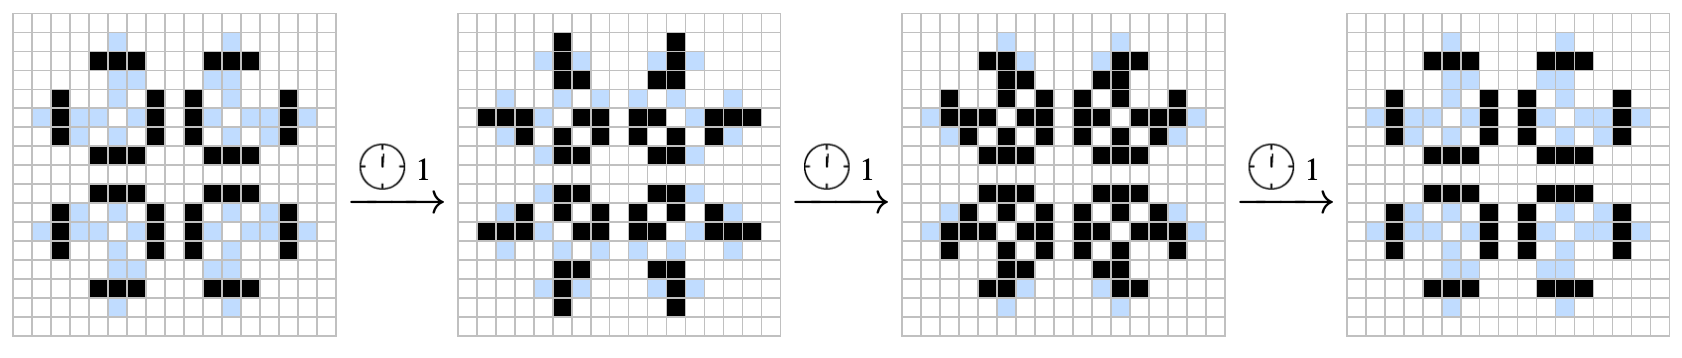
\includegraphics[width=14cm]{figure_three.png}
    \caption{Period 3 Oscillator known as a Pulsar}
    \text{Nathaniel Johnston and Dave Greene. Conway’s Game of Life: Mathematics and Construction.}
    \cite{JG2022conway}
\end{figure}




  \item \textbf{Spaceship: } \\ A pattern that returns to its initial phase after it completes its period, but ends in a different location from where it started. \cite{JG2022conway}
\end{enumerate}

 \begin{figure}[ht]
          \centering
    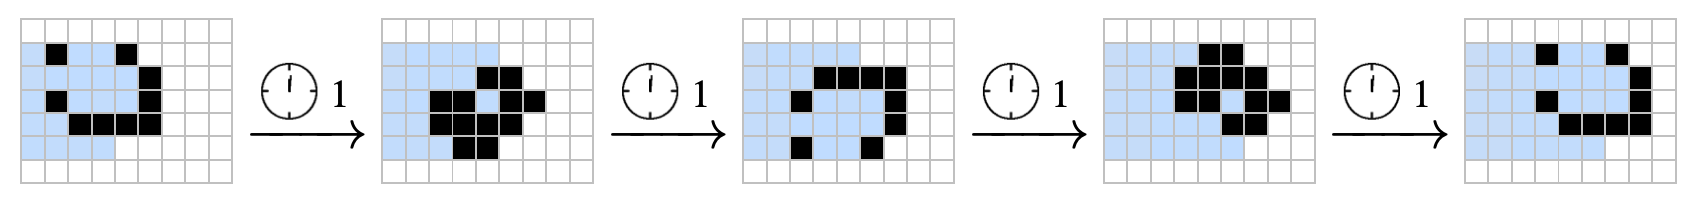
\includegraphics[width=15cm]{figure_four.png}
    \caption{Period 4 Spaceship which moves orthogonally across the grid}
    \text{Nathaniel Johnston and Dave Greene. Conway’s Game of Life: Mathematics and Construction.}
    \cite{JG2022conway}
\end{figure}


In defining the following life-forms, the next natural question to ask is: \textit{Given an initial starting configuration is it possible to decide if any Still Life, Oscillator, or Spaceship life-form patterns are reachable in t many generations?}

\

This question can be distilled down into a particular instance of the Pattern Reachability Problem (PREP) \cite{SUTNER199587}. The Pattern Reachability Problem asks: 

 \

 \textit{Question: } Given some instance of Conway's Game of Life, a cellular automata \textbf{GoL} [see \ref{gol}], a source configuration $X$ and a target configuration \textbf{$X_0$}, \textit{is there some configuration in the orbit of X that matches $X_0$, given $t$ generations pass?} \cite{SUTNER199587}.

\subsection{Definitions, Theorems, and other Important Terminology}
Before proving the proposition that 
\textit {PREP can be decided in nondeterministic polynomial time for two-dimensional finite automata in Conway's Game of Life} [see \ref{NP_proof}], lets first formulate the necessary definition, encodings, and terminology we'll need moving forward.

\subsection{Encoding cellular automata in Conway's Game of Life}
To begin, let's represent an instance of a cellular automata in Conway's Game of life as a finite string over an alphabet. The following encoding is inspired by \textit{Sutner's} encoding scheme \cite{SUTNER199587}.
\begin{enumerate}
  \item[(a)] Let a CA in \textbf{GoL} be represented as a 4-tuple: \textbf{GoL = } $ <d, k, w, p> $ \label{gol}
    \begin{enumerate}
      \item[-] $d$ denotes the dimensions of the \textbf{finite} grid that the automata evolve in. In representing Conway's game of life, our dimensions space will be set to $d = 2$
      \item[-] Every cell has a finite number of states, let's use a finite alphabet $\Sigma_k$, where $\Sigma_k = \{0,1\}$, $1$ indicating that a particular cell is \textit{living}, and $0$ indicating that that cell is \textit{dead}. Let $k$ represent this alphabet.
      \item[-] Positive integer $w$ represents the width of a automata's neighborhood in \textbf{GoL}, meaning \textit{the automata's direct neighbors that are involved in updating the cell}. Width is a result of the radius relation: $w = 2*r +1$. Within \textbf{GoL}, our neighborhood rules [rule: \ref{rule_one}], indicate $r = 1$, and $w = 3$.
      \item[-] Let $p : \Sigma^N \to \Sigma$ be the local function which expresses the formal rule mapping (or \textit{local rule}) of the automate in Conway's Game of Life. Our set of rules applies directly from the surrounding neighborsA $ N = [-r, r]^d \subseteq \mathbb{Z}^d $, and updates the cell in the center of the neighborhood.
      \item[-] A map $ X : C \to \Sigma $ takes the set $ C $ of all cells and maps to a state $ k \in \Sigma$. X is the \emph{configuration} of the cellular automaton.
    \end{enumerate}
      \item[(b)] The local map $p$ only updates a given automata based on it's direct neighbors. To extend this to the entire configuration $C$, let's define a global mapping $\rho$ which updates all cell simultaneously. This process will utilize our local mapping rule $p$, and  can be broken into two steps: 
        \begin{enumerate}
          \item[1).] For each cell $c \in C$ create it's local configuration $X_c$, which captures the neighbors around $c$.
          \item[2).] Apply the local rule $p$ to $X_c$ to get the new state at $c$.
        \end{enumerate}
        The global update rule $\rho : \Sigma^C \to \Sigma^C$ is  given by:
        \begin {equation}
        \rho(X)(c) = p(X_c)
        \end {equation}
      \item[(c)] In constructing a \textit{finite} instance of Gol, we must consider how cellular automata behavior on boundaries of the grid.
        \begin{enumerate}
          \item[-] To solve this problem, we will adopt \textit{fixed boundary conditions} \cite{SUTNER199587}. We'll assume that all cells that are not represented in our finite grid will have a fixed state set to $0$. In doing so we can redefine our local mapping $p$ slightly: 
          \item[-] Define $X_c(z)$ to be the state of a cell at postion $c + z$, whenever $c + z \in C$, define its state to be 0, if $c + z$ falls outside the grid.
        \end{enumerate}
      \item[(d)] Let's define the formal definition of a \textit{pattern}. \cite{SUTNER199587}
        \begin{enumerate}
           \item[-] A pattern is a partial configuration, defined as a map $X_0: C_0 \to \Sigma$, where $C_0 \subseteq C$.
    \item[-] We say that a configuration $X$ matches pattern $X_0$ if $X(c) = X_0(c)$ for all $c \in C_0$.
        \end{enumerate}

\item[(e)] The \textit{orbit} of a configuration $X$ is another important definition in regard to our Pattern Reachability Question. The \textit{orbit} is the full set of all intermediary states the system ever passes through starting from $X$. Formally, the orbit is defined as

\begin{equation}
  \text{Orbit of } X = \{ X, \rho(X), \rho^2(X), \rho^3(X), \dots \}
\end{equation}

Another, more useful way we'll be using \textit{orbit} will in regard to some $t$ that is: 

\begin{equation}
\text{Orbit}(X) = \{ \rho^t(X) \mid t \geq 0 \}
\end{equation}

where \( \rho \) is the global update rule and \( t \) ranges over the non-negative integers.
\end{enumerate}
\section{Pattern Reachability}
Now that we have built out the formal definition of \textbf{GoL} automata, we can treat the Pattern Reachability question as a decision problem that uses our \textbf{GoL} definitions. To prove that \textbf{PREP} $\in$ \textbf{NP}, let's begin by expressing \textbf{PREP} more formally as a decision problem: \textit{Does there exist a time $t \geq 0$ such that the configuration $\rho^t(X)$ contains a given pattern $X_0$?}

\subsection{PREP is in NP:}

\label{NP_proof}
\textit{Let's prove by constructing a certificate based definition}\\
\\
\textbf{Problem Input:}
\begin{itemize}
  \item An instance of \textbf{GoL} automata: $<d = 2, \Sigma_k = \{0,1\}, w = 3, p = \text{(local rule)}>$
    \item Finite grid configuration $ C$, where $ |C| $ is the total number cells $n$.
  \item Initial configuration $ X: C \to \Sigma_k = \{0,1\}$ 
    \item Target pattern $ X_0: C_0 \to \Sigma_k $ where \( C_0 \subseteq C \)
\end{itemize}

\subsubsection{NP Certificate Based Proof:\cite{SUTNER199587}}
We say a  Language \textbf{L} $\in$ \textbf{NP} if there exists a polynomial-time TM that can verify \textbf{PREP}'s certificate efficiently. Let's begin by constructing the certificate (nondeterministicically guessing the solution to \textbf{PREP}).

\begin{enumerate}
    \item \textbf{Certificate:} A tuple $Z = <t, X_0 >$
      Where: 
      \begin{enumerate}
          \item[(a)] $t$ is a non-negative integer that represents the number of configuration states 
          \item[(b)]) $X_0$ represents the target pattern configuration $\rho^t(X)$ should produce after $t$ configuration states.
      \end{enumerate}
    \item \textbf{Verification process} Given tuple $Z$:
    \begin{enumerate}
        \item Begin by simulating GoL for $t$ steps. Start with configuration $X$, compute $\rho^t(X)$ (the \textit{orbit} of $X$).
        \begin{itemize}
            \item Apply our Local update rule: For each cell $c \in C$, compute its next state based on surrounding neighborhood. Each cell is able to apply the local rule in constant time: $O(1)$
            \item To update all $n$ cells in configuration, this takes $n*O(1)$ or $O(n)$ time. This our ``per-step" time.
            \item Total compute time for $t$ steps is: $O(t * n) = O(n * t)$
        \end{itemize}
        \item Now we must Check to see if resulting configuration matches, that is, we must verify $\rho^t(X)$  matches $X_0$ on $C_0$:
        \begin{itemize}
            \item For each cell $c \in C_0$ check if $\rho^t(X)(c) = X_0(c)$.
            \item This checking must be done for $ |C_0| \leq n $ cells, which takes time: $ O(n) $.
        \end{itemize}
    \end{enumerate}

    \item \textbf{Total verification time: }
      \begin{equation}
        O(t*(n)*n)+O(n)= O(t *n^2) \in \textbf{P} 
    \end{equation}
    \textit{For any} $t$ \textit{in polynomial time}.
  \item[]\textbf{Analysis}
    The orbit of the initial configuration $X$ under repeated application of our global update rule $\rho$ describes all possible future sub-states the configuration. Our certificate claims that at some guessed $t$ value the configuration $\rho^t(X)$ will represent the desired pattern $X_0$. More specifically, since we can compute the orbit in $t$ steps and check if the resulting configuration matches $X_0$ in polynomial time, \textbf{PERN} $\in$ \textbf{NP}.
\end{enumerate}

\subsection{Still Life, Oscillator, and Spaceship Pattern Reachability}

\textbf{Let's now apply the proof above to particular instances of common patterns in GoL}
In any each case we start be expressing the target pattern as a partial configuration
\begin{equation}
  X_0 \colon C_0 \to \{0,1\},
\end{equation}
Our decision question remains the same: $\exists\,t\ge0:\ \rho^t(X)$ produces a configuration ${C_0}$ which is equal to $X_0$?.

\
\

\textbf{Still Life analysis:}
Our proof [\ref{NP_proof}] applies most directly for the still life patterns. That is, we can define our target pattern as one of the particular Still life forms [see figure \ref{stil_lifes}]. 
\[
  \rho(X_0)(c) = X_0(c)\quad\forall\,c\in C_0.
\]

\paragraph{Oscillator (period \(p>1\)).}
\[
  \rho^p(X_0)(c) = X_0(c)
  \quad\text{and}\quad
  \rho^k(X_0)\neq X_0\quad(1\le k<p).
\]

\paragraph{Spaceship (translation \(\mathbf v\), period \(p\)).}
\[
  \rho^p(X_0)(c) = X_0(c - \mathbf v)
  \quad\forall\,c\in C_0.
\]


\section{What can be computed/decided in Conway’s Game of Life?}

\section{REACHES-CONFIGURATION is undecidable}

\printbibliography

\end{document}
